\documentclass[aspectratio=169]{beamer}

%%\usepackage{qfdslides}
\usepackage{hjsslides}
\usepackage{grffile}

\hypersetup{colorlinks,urlcolor=blue}

\newcommand{\startsection}[2][]{%
\ifnum\pdfstrcmp{#1}{}=0
\section{#2}
\else
\section[#1]{#2}
\fi
\begin{frame}{#2}
  %% \begin{minipage}{\textwidth}
    \tableofcontents[currentsection,hideothersubsections]
  %% \end{minipage}
\end{frame}
}

\bibliography{bibliography}


\title{COVID-19: The Data Abuse Pandemic}

\author[Harvey J. Stein]{Harvey J. Stein\\\texttt{hjstein@bloomberg.net}}
\institute[Bloomberg LP]
{
  Head, Quantitative Risk Analytics\\
  Bloomberg L.P.
}


\date{Bloomberg Quant Seminar\\
  May, 2020\\
  DRAFT SLIDES}

\begin{document}

\nocite{nyc2020data,Stein2020nycdata,Stein2020owiddata,owid2020data}
\nocite{Stein2020Seem,Stein2020Ray,owid2020data,JHU2020data}
\nocite{NYT2020data}

\parskip=.4em plus .6em minus .4em

\begin{frame}

  \titlepage

\blfootnote{If errors are found, please return them to {\tt hjstein@bloomberg.net}.}

\end{frame}

\begin{frame}{What they first showed in NYC}
  \begin{figure}
    \centering
%    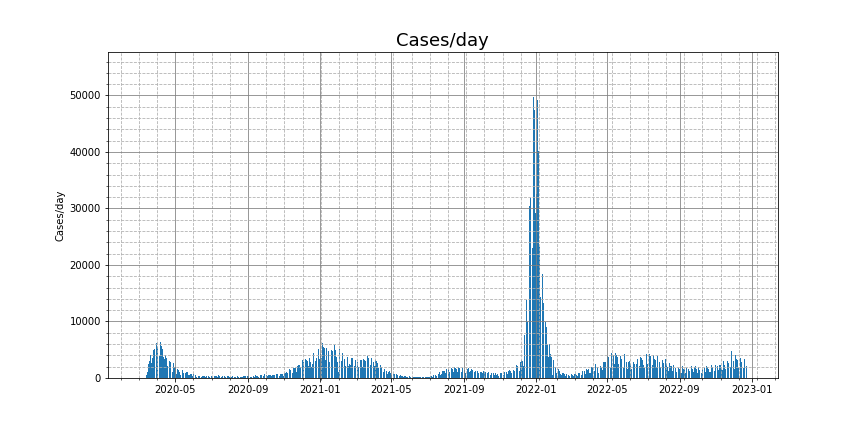
\includegraphics[width=1\textwidth]{../Notebooks/whatTheyTellYou.png}
%    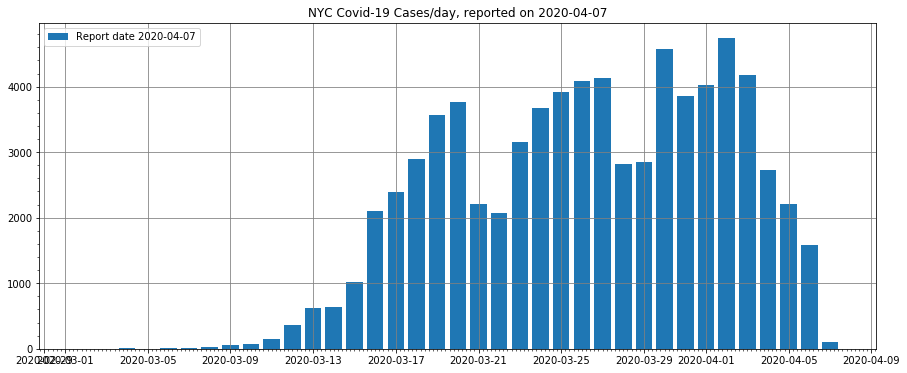
\includegraphics[width=1\textwidth]{../Notebooks/casesPerDay2020-04-07T17_52_37.000000000.png}
    \includegraphics[width=1\textwidth]{../Notebooks/casesPerDay2020-03-26T11_26_41.000000000.png}
  \end{figure}
  Looks like cases/day are dropping off after 3/20
\end{frame}

\begin{frame}{Eight days later}
  \begin{figure}
    \centering
%    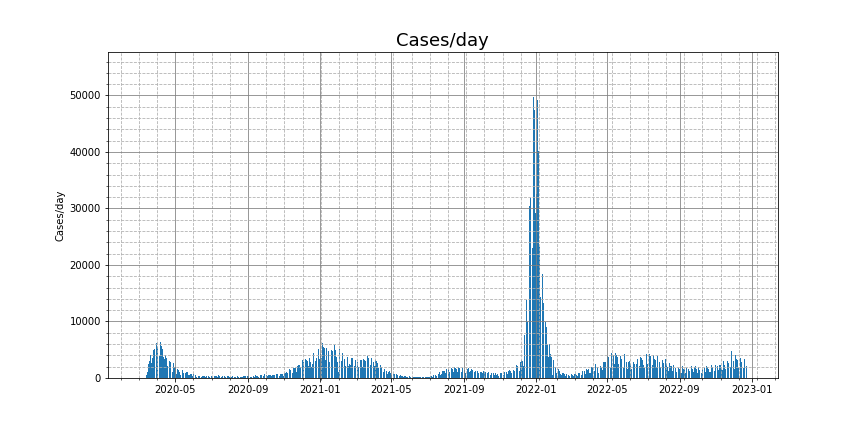
\includegraphics[width=1\textwidth]{../Notebooks/whatTheyTellYou.png}
%    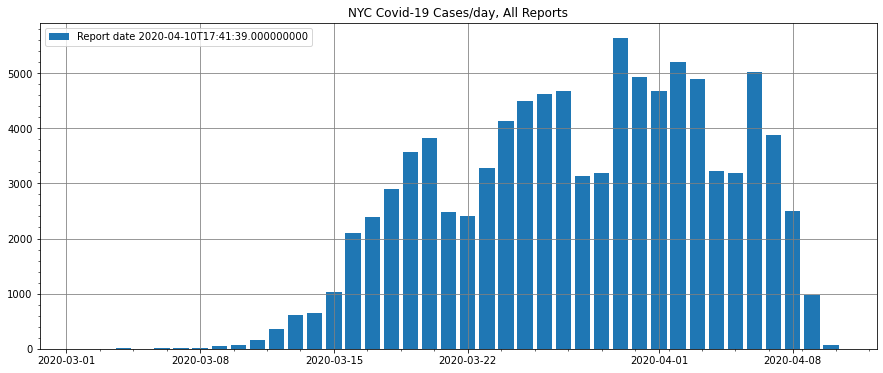
\includegraphics[width=1\textwidth]{../Notebooks/casesPerDay2020-04-10T17_41_39.000000000.png}
    \includegraphics[width=1\textwidth]{../Notebooks/casesPerDay2020-04-03T18_15_27.000000000.png}
  \end{figure}
  Now it looks like cases/day are \alert{rising} through 3/30!
\end{frame}

\begin{frame}{What they didn't say}
  \begin{figure}
    \centering
    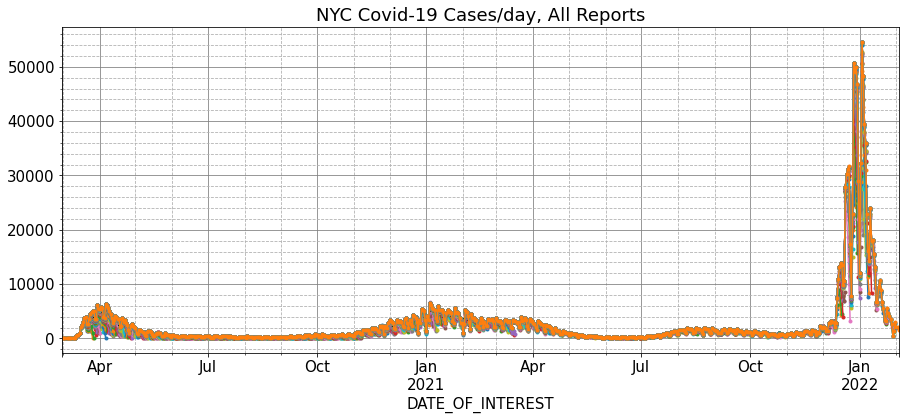
\includegraphics[width=.9\textwidth]{../Notebooks/theFullStory.png}
  \end{figure}
  Since April 12th, every report has peaked on April 6th
\end{frame}

\begin{frame}{After appropriate smoothing}
  \begin{figure}
    \centering
    \includegraphics[width=.9\textwidth]{../Notebooks/fullNYCSmoothed.png}
  \end{figure}
  Since April 13th, every smoothed report has peaked on April 8th
\end{frame}

\begin{frame}{Abuses}
  What's going on?
  \begin{itemize}
  \item Different sites report cases at different times
  \item Large dip in confirmed cases every weekend
  \end{itemize}
  
  Impact:
  \begin{itemize}
  \item Reporting delays can account for 30\% changes as much as 3
    weeks later
  \item Latest counts for each date are reported -- history is harder
    to extract
  \item Low weekend counts obscure trends -- need to use 7 day rolling
    average
  \item Reporting aggregates instead of per site data makes analysis difficult
  \end{itemize}

But this is the good case!

See:
\begin{itemize}
\item \citewt{Stein2020Ray}
\item \citewt{Stein2020Seem}
\end{itemize}
\end{frame}

\begin{frame}{What they said for the USA}
  \begin{figure}
    \centering
    \includegraphics[height=.7\textheight]{../Notebooks/USACasesPerDayLatestRawNoLegend.png}
  \end{figure}
  What happened to the weekend dip?
\end{frame}


\begin{frame}{What they didn't say}
  \begin{figure}
    \centering
    \includegraphics[height=.7\textheight]{../Notebooks/USACasesPerDayHistoryRawNoLegend.png}
  \end{figure}
  Where are the data updates?
\end{frame}


\begin{frame}{Abuses}
  What's going on?
  \begin{itemize}
  \item Recording by report date instead of by incident date!
  \end{itemize}
  
  Impact:
  \begin{itemize}
  \item No record of when incidents actually occurred
  \item Misstates ramp up to peak, delays peak and overstates
    post-peak incidents
  \item Obscures periodicity and adds noise
  \item Makes modeling harder and more error prone
  \item News reports of yesterday's numbers are deceptive
  \end{itemize}

  Recording by report date is rampant -- all major sources do it:
  \begin{itemize}
  \item \href{https://github.com/owid/covid-19-data}{Our World in Data
    repository} (data from the European CDC)
  \item \href{https://github.com/CSSEGISandData/COVID-19}{Johns Hopkins
    University COVID-19 repository}
  \item \href{https://github.com/nytimes/covid-19-data}{New York Times
    COVID-19 repository}
  \end{itemize}
\end{frame}

\begin{frame}{Impact}
  \begin{figure}
    \centering
    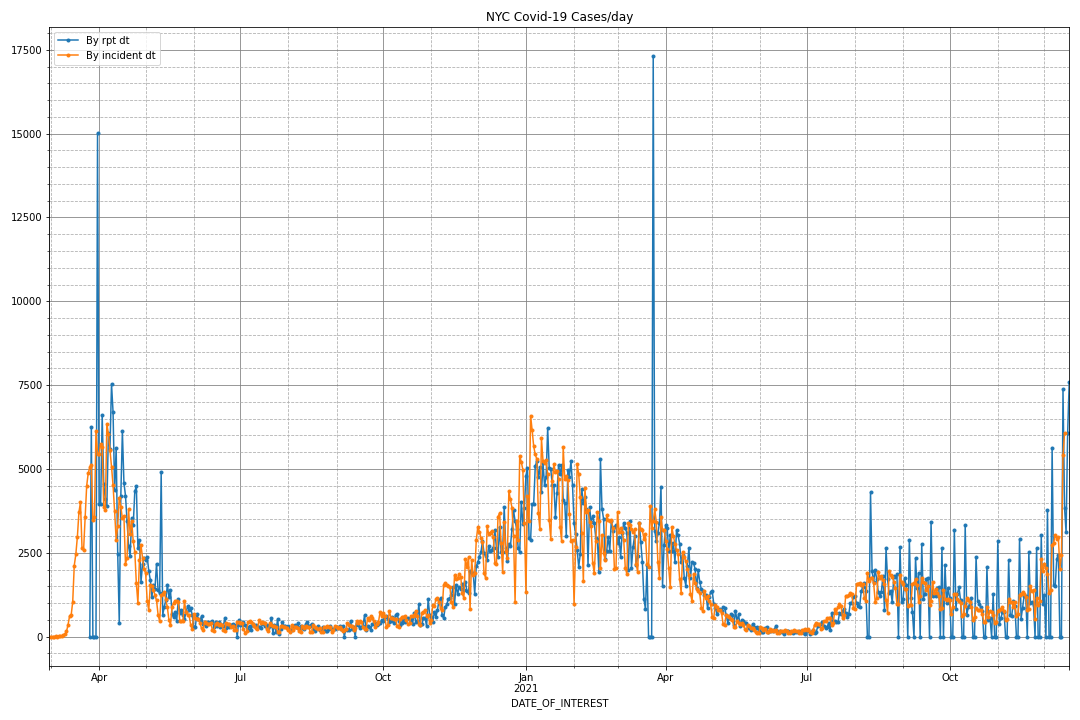
\includegraphics[height=.8\textheight]{../Notebooks/casesPerDayHistoryRptDtVsInDtRaw.png}
  \end{figure}
\end{frame}

\begin{frame}{Impact}
  \begin{figure}
    \centering
    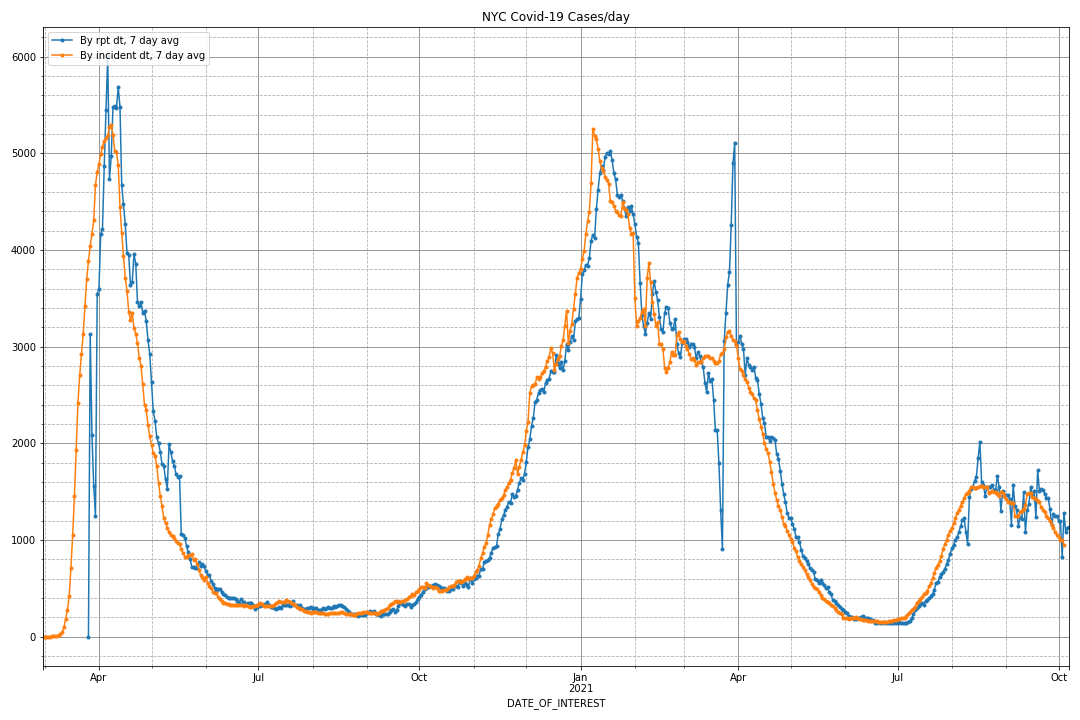
\includegraphics[height=.8\textheight]{../Notebooks/casesPerDayHistoryRptDtVsInDt.png}
  \end{figure}
\end{frame}

\begin{frame}{Summary}
  What now?
  \begin{itemize}
  \item Know your data!
  \item Be aware that recent reports are inaccurate -- either missing
    data or misrepresenting counts
  \item Account for this in your modeling
  \item Ask data sources to collect by incident date, publish full
    history and publish per site data instead of aggregating
  \item Investigate actual meaning of data -- classification of COVID-19
    hospitalizations, deaths due to COVID-19, ...
  \end{itemize}

  See \citewt{Stein2020Garbage}) 
\end{frame}

\begin{frame}[allowframebreaks]
  \frametitle{References}
  \label{refs}
  \begin{small}
  \printbibliography
  \end{small}
\vfil
%\vbox{\hbox{\tiny{\copyright~Bloomberg Finance L.P. All rights reserved.}}
\vbox{\hbox{}
%% ~\hskip -1.5em\hbox to \hsize{%
%%   \includegraphics[width=\hsize,keepaspectratio=true]{legalfooter.eps}}%
}%
\end{frame}

\end{document}
